\section{ Pengertian MapServer}

MapServer adalah sebuah aplikasi pengembangan yang bersifat terbuka (open source) untuk pengembangan aplikasi internet yang melakukan pengolahan spasial. Bisa dijalankan sebagai sebuah program CGI atau Mapscript yang mendukung beberapa bahasa pemrograman.
MapServer adalah aplikasi Open Source yang memungkinkan suatu data peta diakses melalui web. Teknologi mapserver pertama kali dikembangkan oleh Universitas Minesotta Amerika Serikat. Dengan adanya MapServer menjadikan pekerjaan membuat Peta Digital menjadi lebih mudah dan interaktif. Maksud dari Interaktif peta disini diartikan bahwa user dapat dengan mudah mengubah dan melihat tampilan peta seperti memperbesar atau memperkecil gambar, rotate, dan menampilkan informasi (seperti menampilkan info jalan) dan analisis pada permukaan geografi. 
MapServer merupakan sebuah program aplikasi GIS berbasis web yang open source. MapServer juga dikembangkan tanpa tujuan komersial, sehingga pengguna MapServer dapat menggunakan dan mengembangkan program MapServer. 
Mapserver merupakan aplikasi freeware dan open source yang meungkinkan kita menampilkan dataspasial (peta) dalam platform web.Aplikasi ini pertama kali dikembangkan oleh Universitas Minesota, Amerika Serikat untuk proyekFor Net (sebuah proyek untuk sumber daya alam )yang disponsori oleh NASA (National Aeronauticsand Space Administration) Support NASA dilanjutkandan dikembangkan proyek TerraSIP  untuk manajemendata lahan. Saat ini sifatnya yang terbuka (open source), pengembangan suatu mapserver dilakukan oleh pengembang dari berbagai Negara. 
Pada bentuk yang paling dasar (based), MapServer berupa sebuah  program CGI (Common Gateway Interface). Program Mapserver tersebut dieksekusi pada sebuah webserver dengan konfigurasi peta yang disimpan dalam sebuah file \*.MAP, kemudian kirim dan ditampilkan oleh web browser baik dalam bentuk gambar peta atau  bentuk yang lain. 

\section{Fitur MapServer}
Ada beberapa fitur utama yang ada dalam mapserver untuk mendukung fungsi sebagai server GIS berbasis web antara lain adalah :
\begin{enumerate}
\item Menampilkan data spasial dalam format vector seperti : Shapefile (ESRI), ArcSDE (ESRI), PostGis dan berbagai format data vector lain dengan dukungan penggunaan library OGR. 
\item Menampilkan data dalam format raster yaitu TIFF/GeoTIFF, EPPL7 dan berbagai format lain dengan menggunakan library GDAL.
\item Menggunakan Quadtree dalam index data, sehingga operasi tersebut cepat dilakukan. 
\item Dapat dikembangkan, dengan tampilan keluaran yang dapat diatur menggunakan file-file template.
\item Dapat melakukan seleksi obyek berdasar nilai, titik, area, atau berdasar sebuah obyek spesial tertentu.
\item Mendukung rendering  karakter berupa font TrueType. 
\item Mendukung penggunaan data raster maupun vector dengan mode tiled (dibagi bagi menjadi sub bagian yang lebih kecil sehingga proses untuk mengambil data dan menampilkan dapat dipercepat).
\item Dapat menggambarkan bagian - bagian  peta secara otomatis, skala grafis, peta indeks maupun legenda peta.
\item Dapat menggambarkan peta tematik yang dibangun menggunakan ekspresi lojik maupun ekspresi regular.
\item Dapat menampilkan label dari objek spasial, dengan label dapat diatur sedemikian rupa, sehingga tidak saling tumpang tindih.
\item Melalui parameter yang ditentukan pada URL konfigurasi diatur secara on the fly  
\item Dapat menangani beragam sistem proyeksi dalam jaringan internet. 
\end{enumerate}

\section{Arsitektur MapServer}
 Secara umum model arsitektur yang digunakan oleh mapserver dapat dilihat pada gambar \ref{arsitektur_map_server} sebagai berikut:

\begin{figure}[ht]
\centering
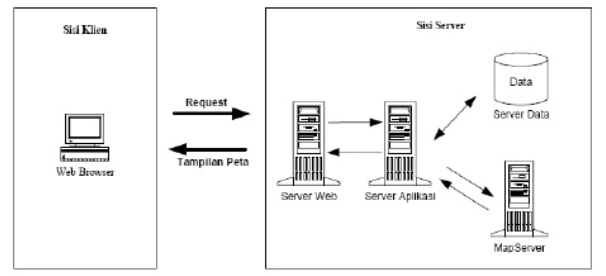
\includegraphics[width=1\textwidth]{pictures/arsitektur_map_server}
\caption{Arsitektur Map Server}
\label{arsitektur_map_server}
\end{figure}

Pola interaksi yang digunakan antara klien dan server berdasarkan skenario request dan respon. Web browser di sisi klien mengirim request ke server web.Karena server web tidak memiliki kemampuan untuk memproses data spasial maka request berkaitan dengan pemrosesan peta akan dikerjakan oleh mapserver sesuai dengan register yang diberikan oleh web server terkait alokasi task dan resource.
Hasil dari pemrosesan yang sudah dilakukan akan di replay melalui server web yang dibungkus dalam sebuah file dalam bentuk HTML atau applet

Mapserver menggunakan pendekatan thin client.
Semua pemrosesan dilakukan di sisi server. Informasi peta dikirimkan ke web browser di sisi klien dalam bentuk file gambar (JPG, PNG, GIF atau TIFF). Kelebihan aplikasi dengan konsep thin client ini adalah sudah beragamnya aplikasi pendukung dalam bentuk framework jadi seperti Chameleon atau cartoweb \cite{walter2018web}


\subitem \textbf{Thin Client}
\begin{enumerate}
\item Fokus pada sisi server.
\item Sebagian besar proses dan analisis data dilakukan berdasarkan request di sisi server.
\item Hasilnya nanti dikirimkan ke klien dalam format standard HTML, yang di dalamnya terdapat file gambar dalam format standard (misalnya GIF, PNG atau JPG)
\item Kelemahan utama pendekatan tersebut menyangkut keterbatasan interaksi opsi dengan user yang kurang fleksibel.
\end{enumerate}

\section{Komponen Teknis}
Komponen yang ada pada sebuah aplikasi GIS mempunyai fungsi utama untuk membaca dan menulisdata spasial, baik yang tersimpan dalam sebuahshapefile (*.shp) atau tersimpan ke dalam sebuah database (Eddy 2006).
Dalam MapServer yang sudah berjalan ada beberapa Komponen utama yang digunakan secara peneuh untuk menjalankan Aplikasi GIS untuk menangani data spasial baik yang tersimpan dalam sebuah flat file atau juga dalam DBMS yaitu :
\begin{enumerate}
\item SHAPELIB
\subitem Shapelib merupakan library yang ditulis menggunakan bahasa pemrograman C yang digunakan untuk melakukan proses read terhadap Shapefile (*.shp) yang sudah didefinisikan. 

\item ESRI (Environmental System Research Institute)
\subitem Format dalam shapefile umum digunakan untuk menyimpan data vector simple (tanpa topologi) dengan atribut, shapefile merupakan format data default yang digunakan dalam GIS.2.

\item GDAL (Geographic Data Abstraction Library) 
\subitem merupakan library yang berfungsi sebagai penerjemah untuk berbagi format data raster, dan sangat dimungkinkan untuk semua abstraksi dari semua data format yang didukung, sehingga beragam format data yang ada akan menghasilkan satu format baku yang dapat digunakan untuk pengembang dalam menampilkan bentuk/format peta yang sesuai semisal akses data untuk direpresentasikan dalam (.gif), (.tif), (.img), (.adf), (.hdrdst3).
\end{enumerate}


